
%(BEGIN_QUESTION)
% Copyright 2011, Tony R. Kuphaldt, released under the Creative Commons Attribution License (v 1.0)
% This means you may do almost anything with this work of mine, so long as you give me proper credit

A gravel-crushing operation uses three long conveyor belts to move rock from the quarry to the crusher.  The belts must be started up in a particular sequence to avoid overloading the electric motors driving them:

$$\includegraphics[width=15.5cm]{i04428x01.eps}$$

First, determine a start-up sequence that makes sense: which conveyor belt should start first, next, and last?  What might happen if the sequence were reversed?  Why not simply start all conveyor motors simultaneously?

\filbreak

This operation uses a Siemens S7 series PLC to control the three conveyor belts.  Analyze this program and explain how it accomplishes the task of starting up the three conveyors in sequence:

$$\includegraphics[width=10.5cm]{i04428x02.eps}$$

Lastly, determine where you might add a contact instruction for an {\it emergency shutoff} safety switch, so that all three conveyors stop simultaneously if ever the safety switch is actuated.

\vskip 20pt \vbox{\hrule \hbox{\strut \vrule{} {\bf Suggestions for Socratic discussion} \vrule} \hrule}

\begin{itemize}
\item{} How long is the time delay between conveyor start-ups?  How might this time delay be altered if needed?
\item{} Suppose a warning siren were added to the system, sounding for a full 15 seconds before the first conveyor belt starts.  How would you modify the PLC program to include this additional functionality?
\item{} Suppose a technician uses the PLC's {\it force} utility to force bit {\tt T2} to a ``0'' state.  How will this affect the operation of the system?  Could the consequences of this force be dangerous in any way?
\item{} Suppose a technician uses the PLC's {\it force} utility to force bit {\tt Q0.1} to a ``0'' state.  How will this affect the operation of the system?  Could the consequences of this force be dangerous in any way?
\end{itemize}

\underbar{file i04428}
%(END_QUESTION)





%(BEGIN_ANSWER)

Although starting all three conveyor motors simultaneously would be very simple, it would be a bad thing to do because of the {\it inrush current} of all three motors placing undue load on the power system.

%(END_ANSWER)





%(BEGIN_NOTES)

Conveyor C starts immediately, followed by conveyor B 8.5 seconds later, followed by conveyor A 8.5 seconds after conveyor B.

\vskip 10pt

An emergency stop input contact could be added in ``series'' with the regular Stop input ({\tt I0.0}).  When the E-stop is pressed, it de-activates {\tt M0.0} and subsequently all timer instructions.

%INDEX% PLC, ladder logic program analysis and explanation

%(END_NOTES)

